\subsubsection{SWITCH} \label{sssec:switch}

Los resultados con conmutación secuencial se muestran en las Figs. \ref{fig:Hval_Switch} a \ref{fig:MP_Switch}.
El valor de entropía calculado para la implementación en punto flotante es $\left \langle H_{hist} \right \rangle = 0.9722$, este valor es ligeramente más alto que el obtenido para el mapa LOG.
Para la aritmética de punto fijo, este valor se alcanza en $B = 24$, pero se estabiliza desde $B = 28$.
En cuanto a los patrones perdidos, el número de MP disminuye a $586$, este valor es menor que el obtenido para el mapa LOG.
Significa que la entropía $H_{BP}$ puede aumentar hasta $\ln(134) / \ln(720) \simeq 0.74$.
Los cuantificadores BP y BPW alcanzan su máximo de $\left \langle H_{BP} \right \rangle = 0.6546$ y $\left \langle H_{BPW} \right \rangle = 0.6313$ a $B = 16$, pero se estabilizan desde $B = 24$.
Las complejidades son menores que para LOG, $\left \langle C_{BP} \right \rangle = 0.4580$ y $\left \langle C_{BPW} \right \rangle = 0.4578$, estos valores se alcanzan para $B \geq 15$ pero se estabilizan en $B \geq 23$.
Comparado con LOG, las propiedades estadísticas son mejores con menos cantidad de bits, para $B \geq 24$ este mapa alcanza mejores características en el sentido de generador aleatorio.

Además, encontramos una condición inicial con un comportamiento anómalo en doble precisión de coma flotante.
Las Figs. \ref{fig:Hval_Switch}, \ref{fig:Hbp_Switch} y \ref{fig:Cbp_Switch} muestran una línea discontinua azul horizontal que está lejos del valor promedio, esto no es detectado por los cuantificadores basados en el procedimiento con contribuciones de ampliotud $BPW$ de las Figs. \ref{fig:Hbpw_Switch} y \ref{fig:Cbpw_Switch}.
Sin embargo, al comparar ambos procedimientos ($BP$ y $BPW$) pudimos detectar una caída a un punto fijo después de un transitorio largo, el procedimiento BPW descarta los valores constantes (que corresponden a un punto fijo) y calcula solo sobre los valores transitorios.
%
\begin{figure}[htpb]
	\centering
	\begin{subfigure}[b]{0.49\textwidth}
		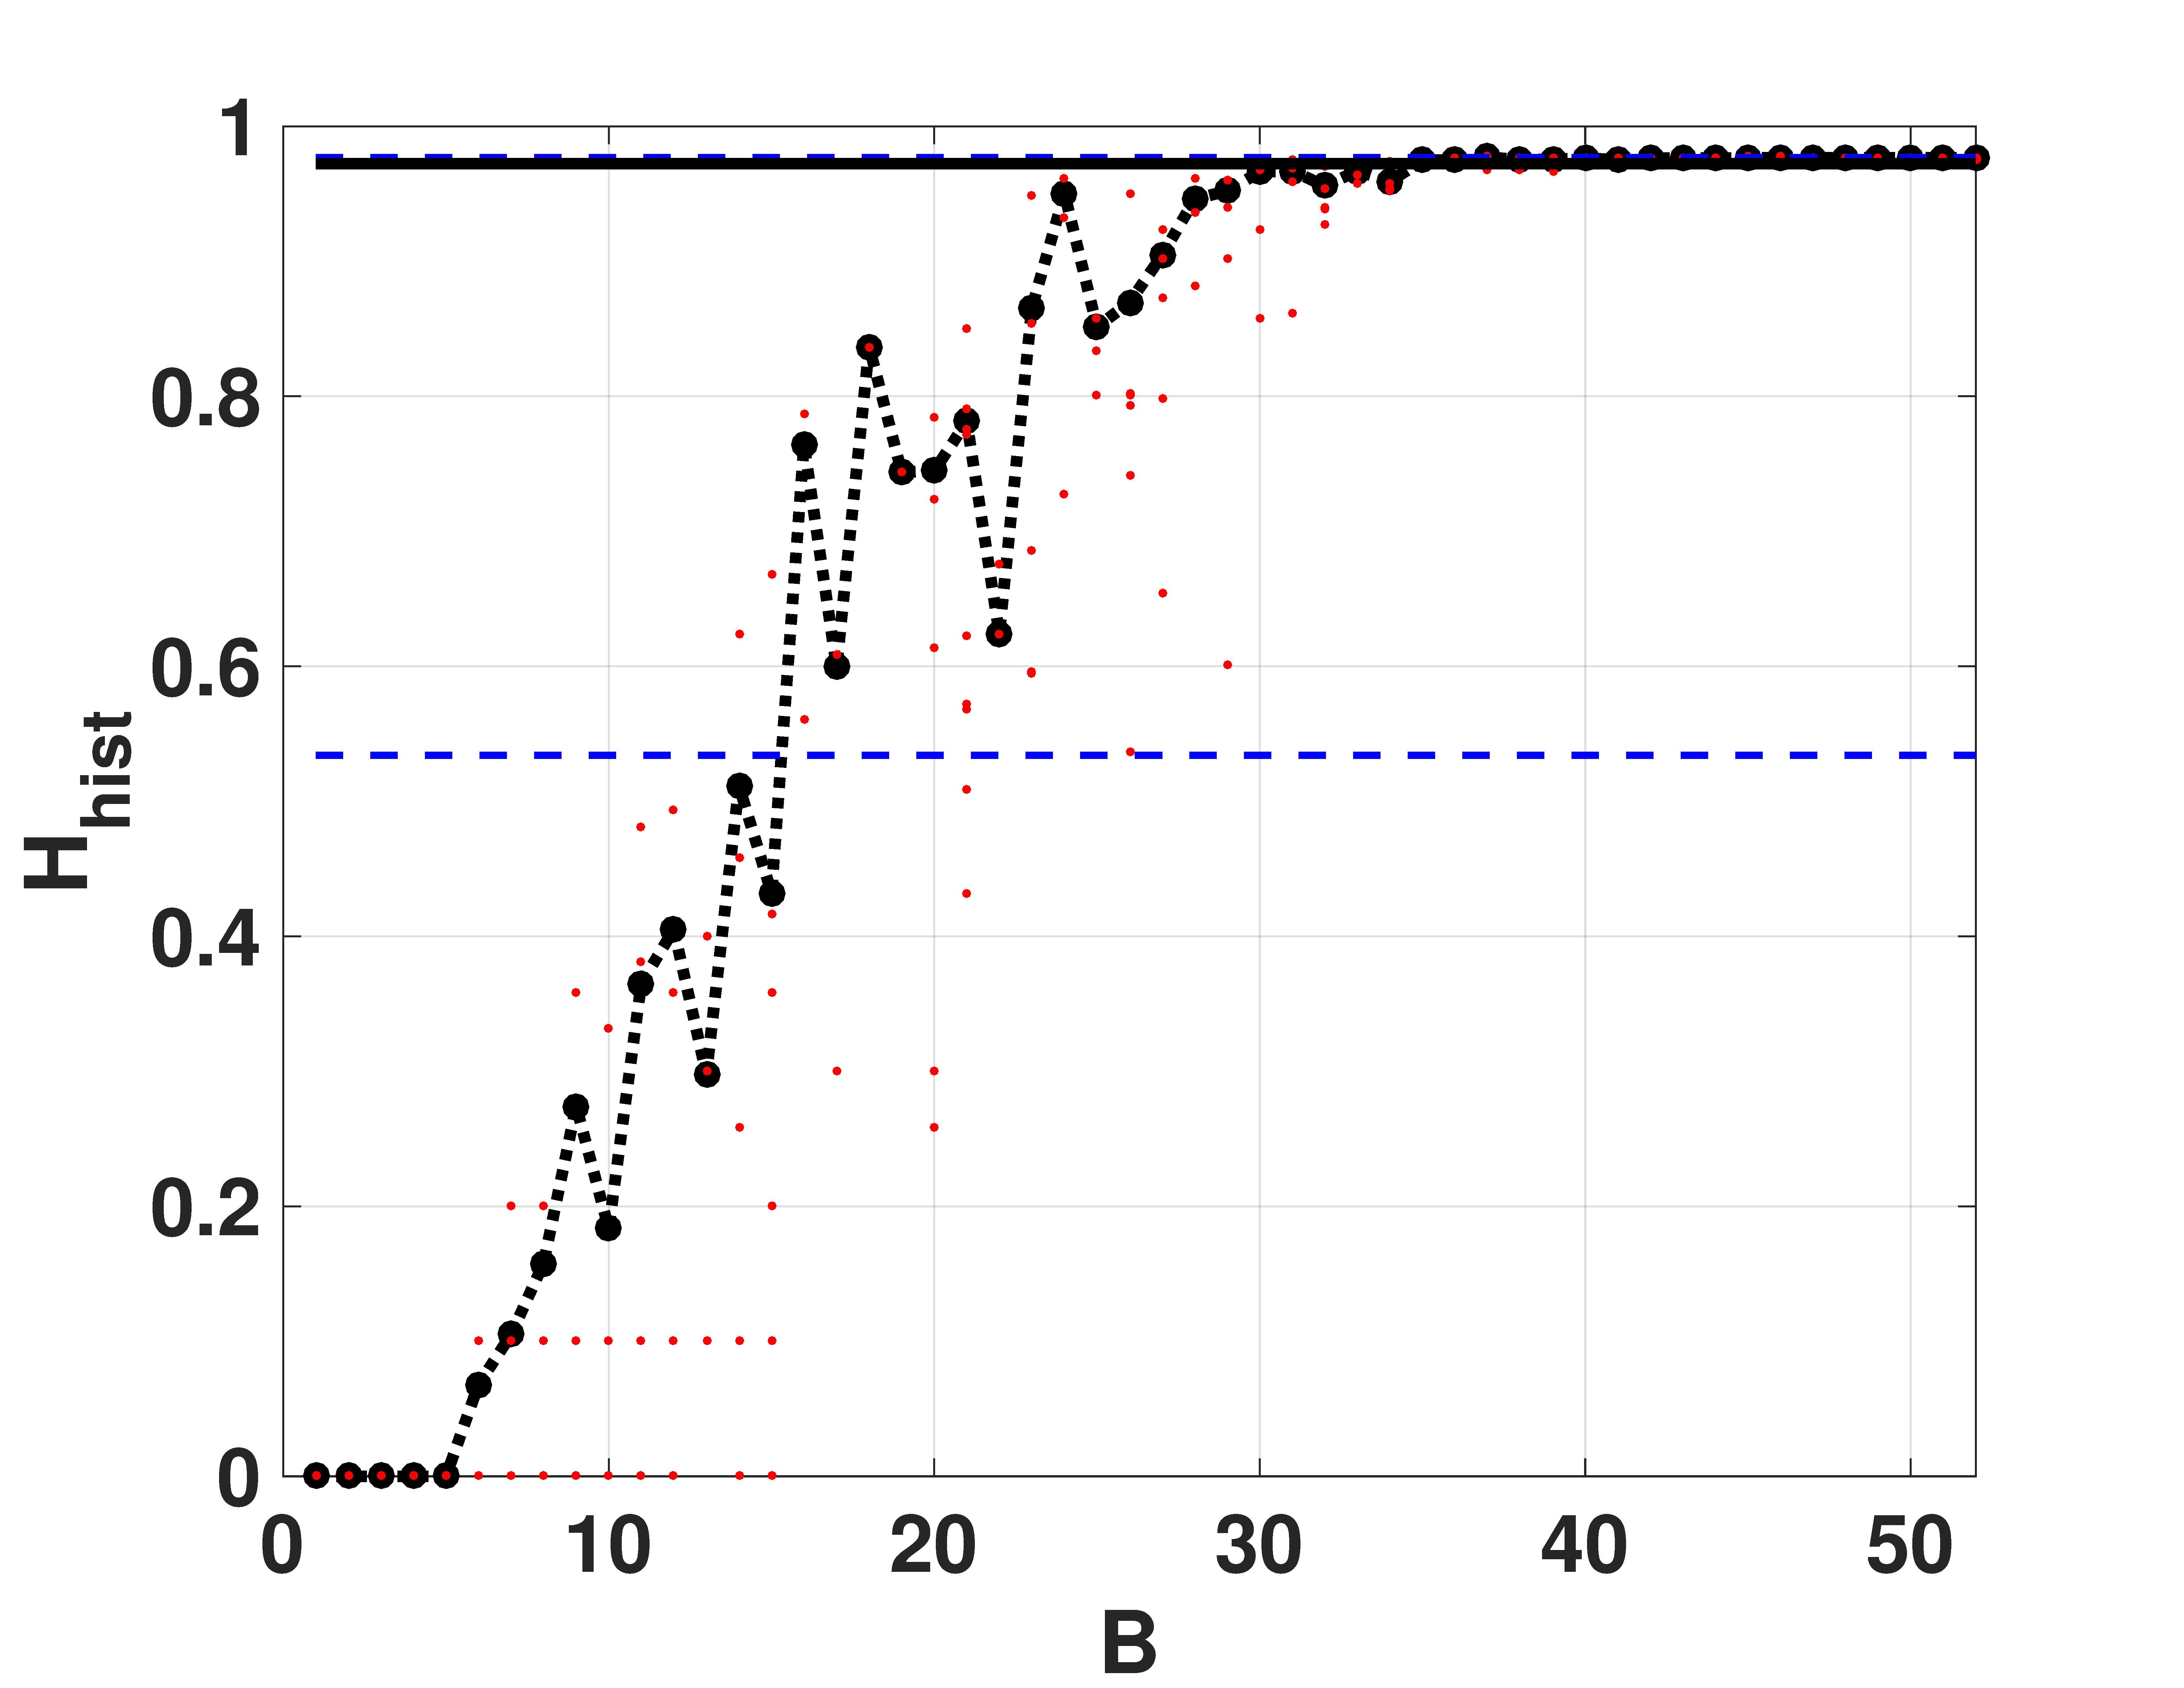
\includegraphics[width=\textwidth]{Hval_Switch}
		\caption{$H_{hist}$ vs. $B$}
		\label{fig:Hval_Switch}
	\end{subfigure}
	\begin{subfigure}[b]{0.49\textwidth}
		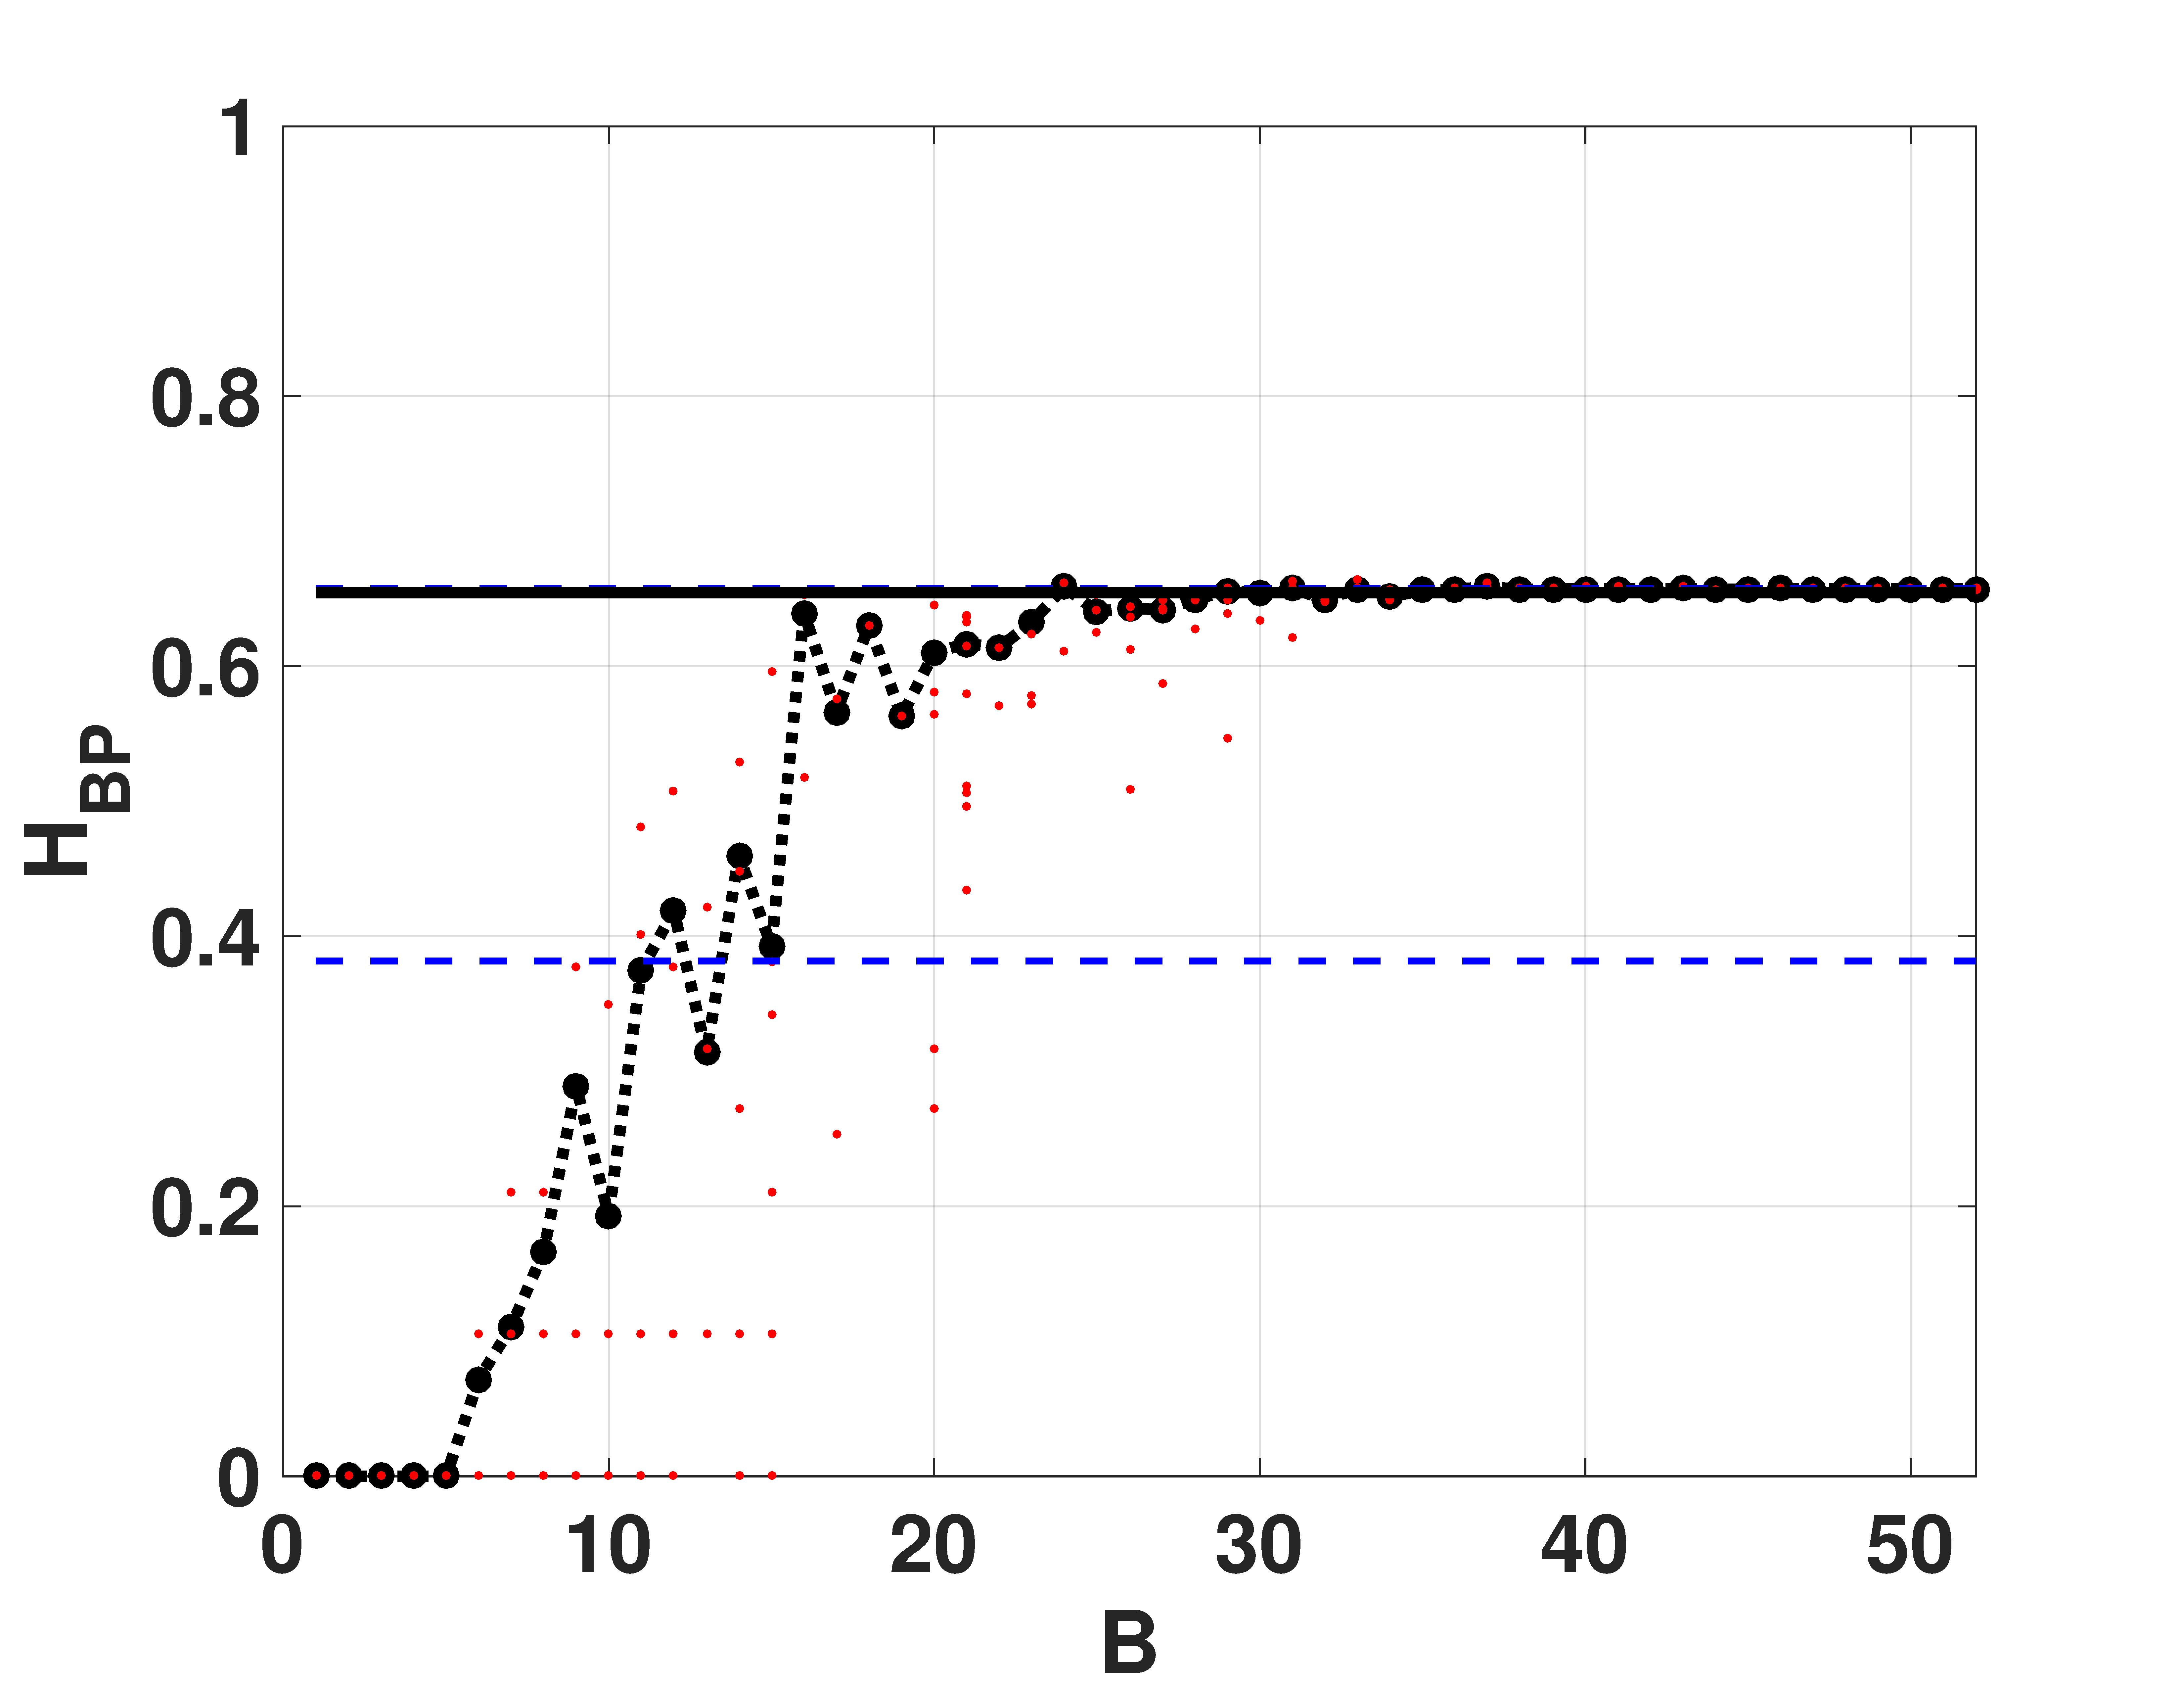
\includegraphics[width=\textwidth]{Hbp_Switch}
		\caption{$H_{BP}$ vs. $B$}
		\label{fig:Hbp_Switch}
	\end{subfigure}
	\begin{subfigure}[b]{0.49\textwidth}
		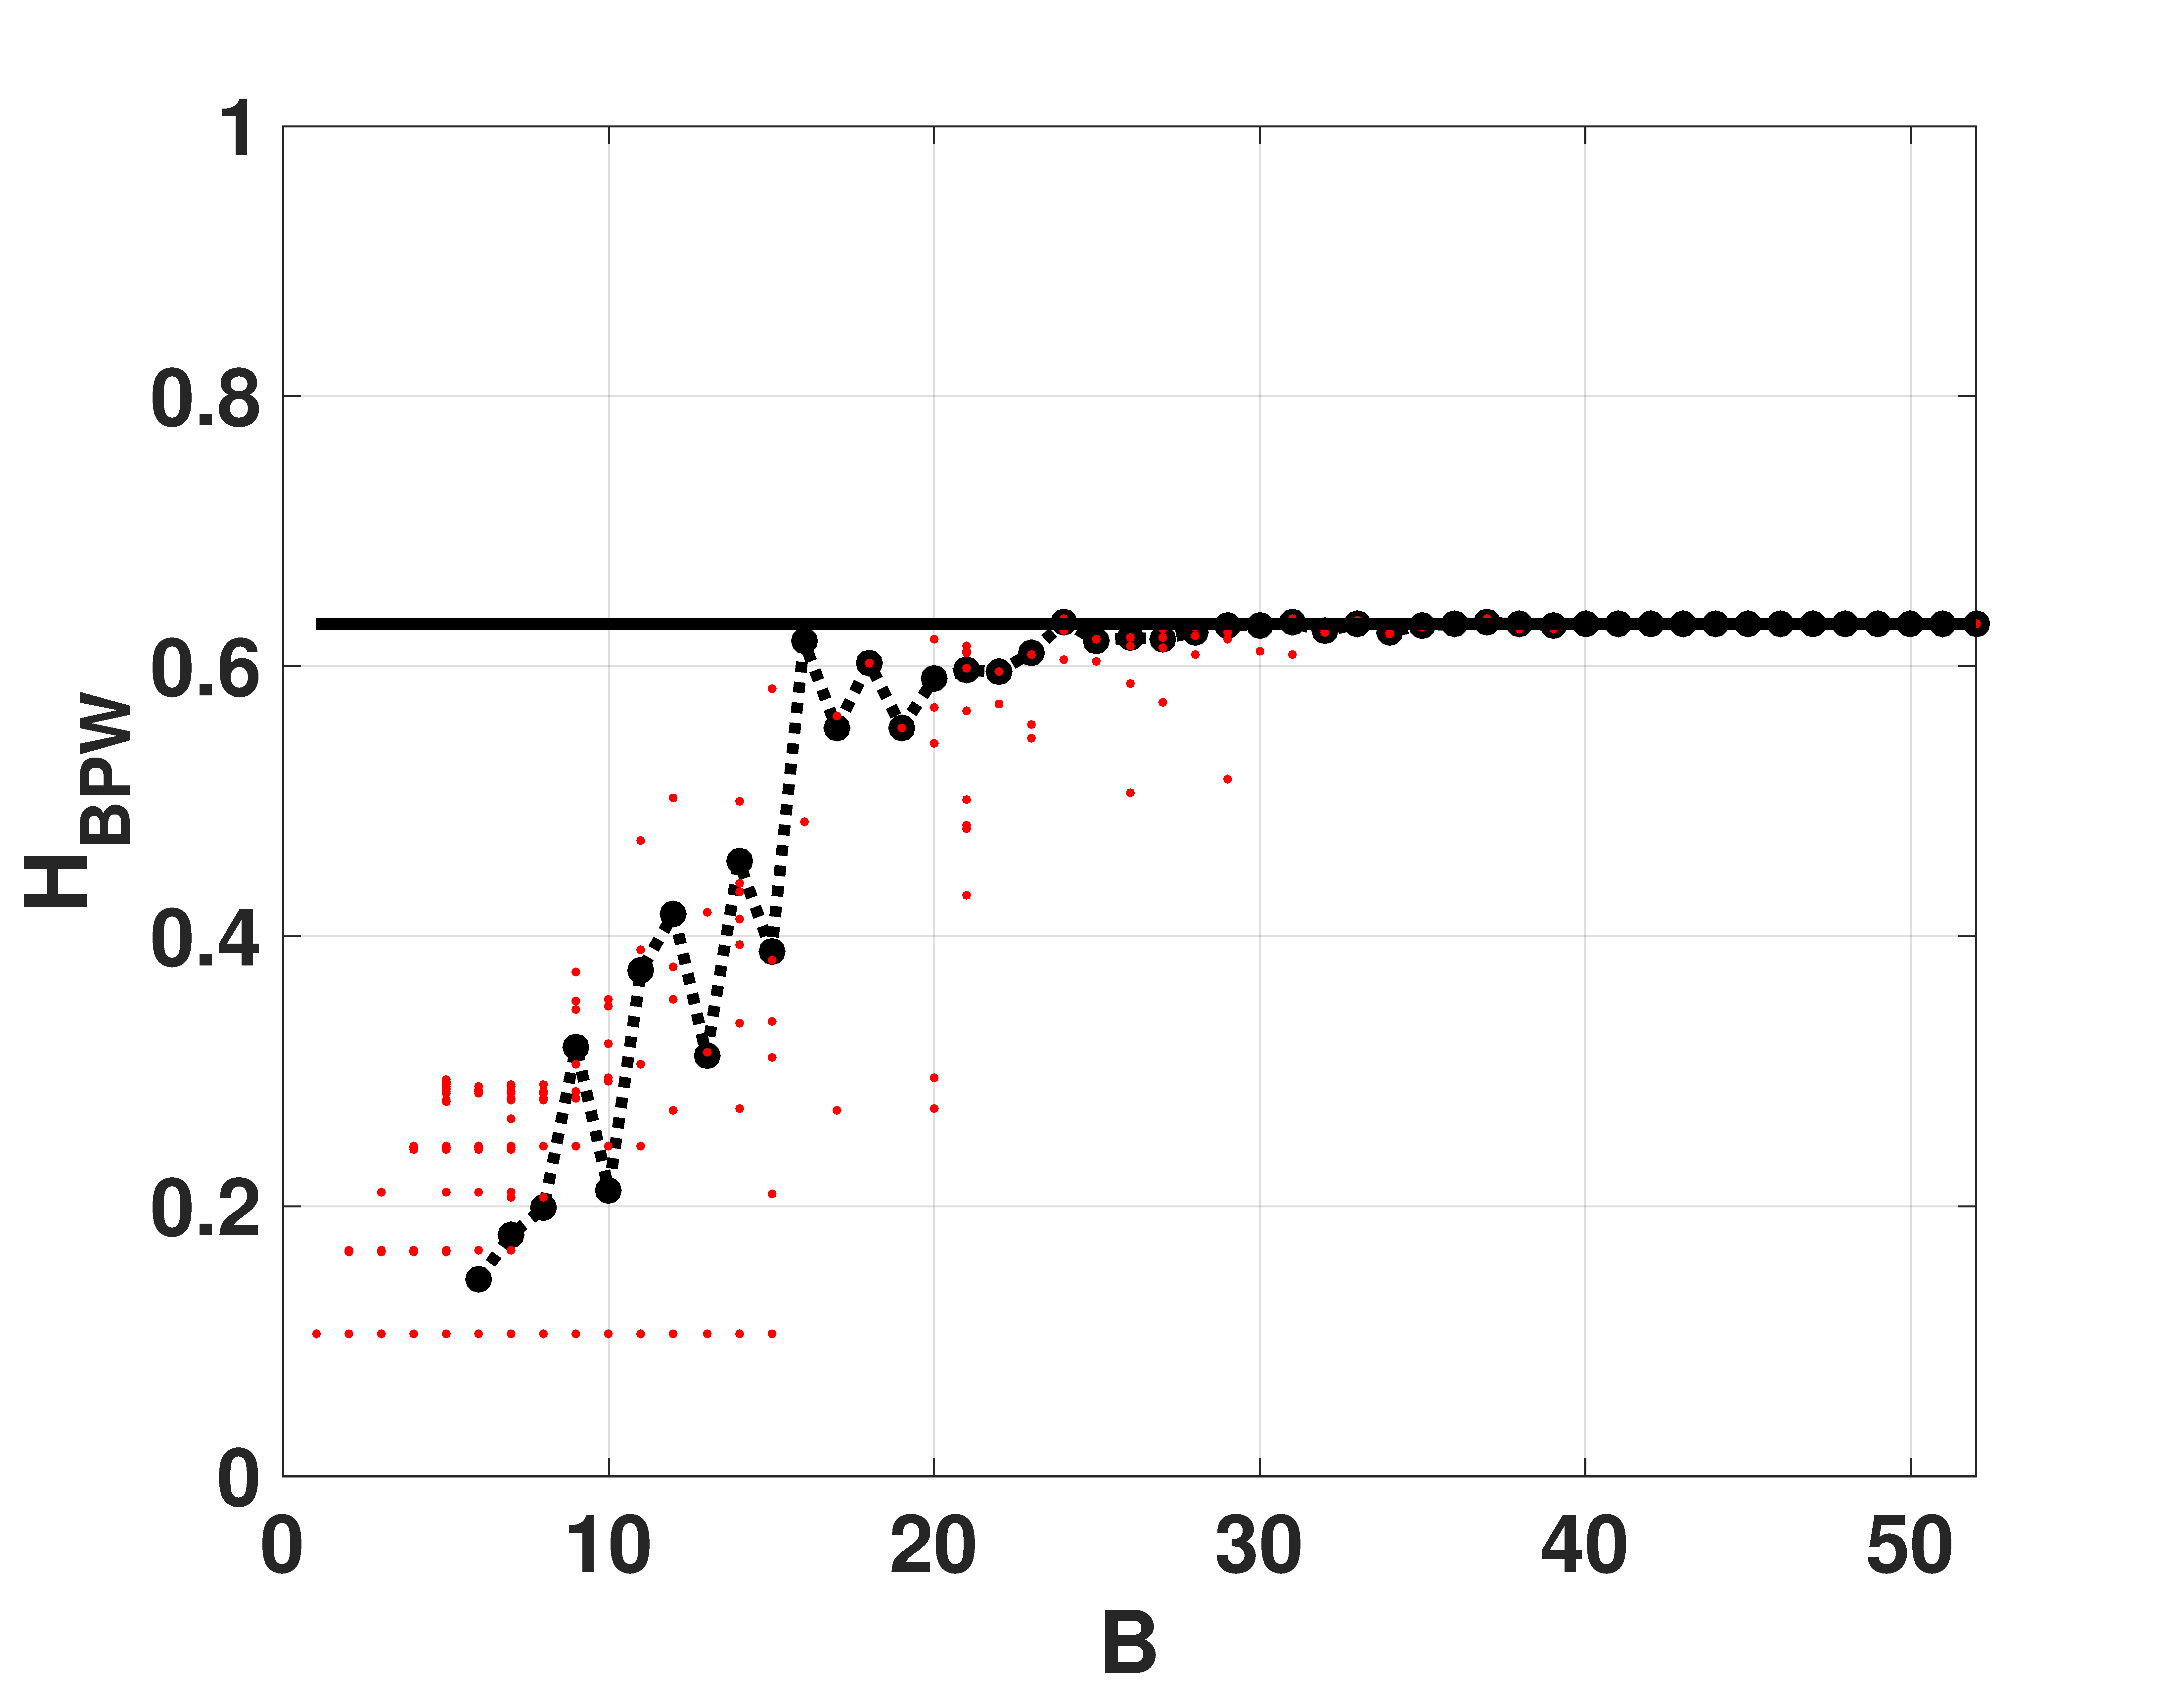
\includegraphics[width=\textwidth]{Hbpw_Switch}
		\caption{$H_{BPW}$ vs. $B$}
		\label{fig:Hbpw_Switch}
	\end{subfigure}
	\begin{subfigure}[b]{0.49\textwidth}
		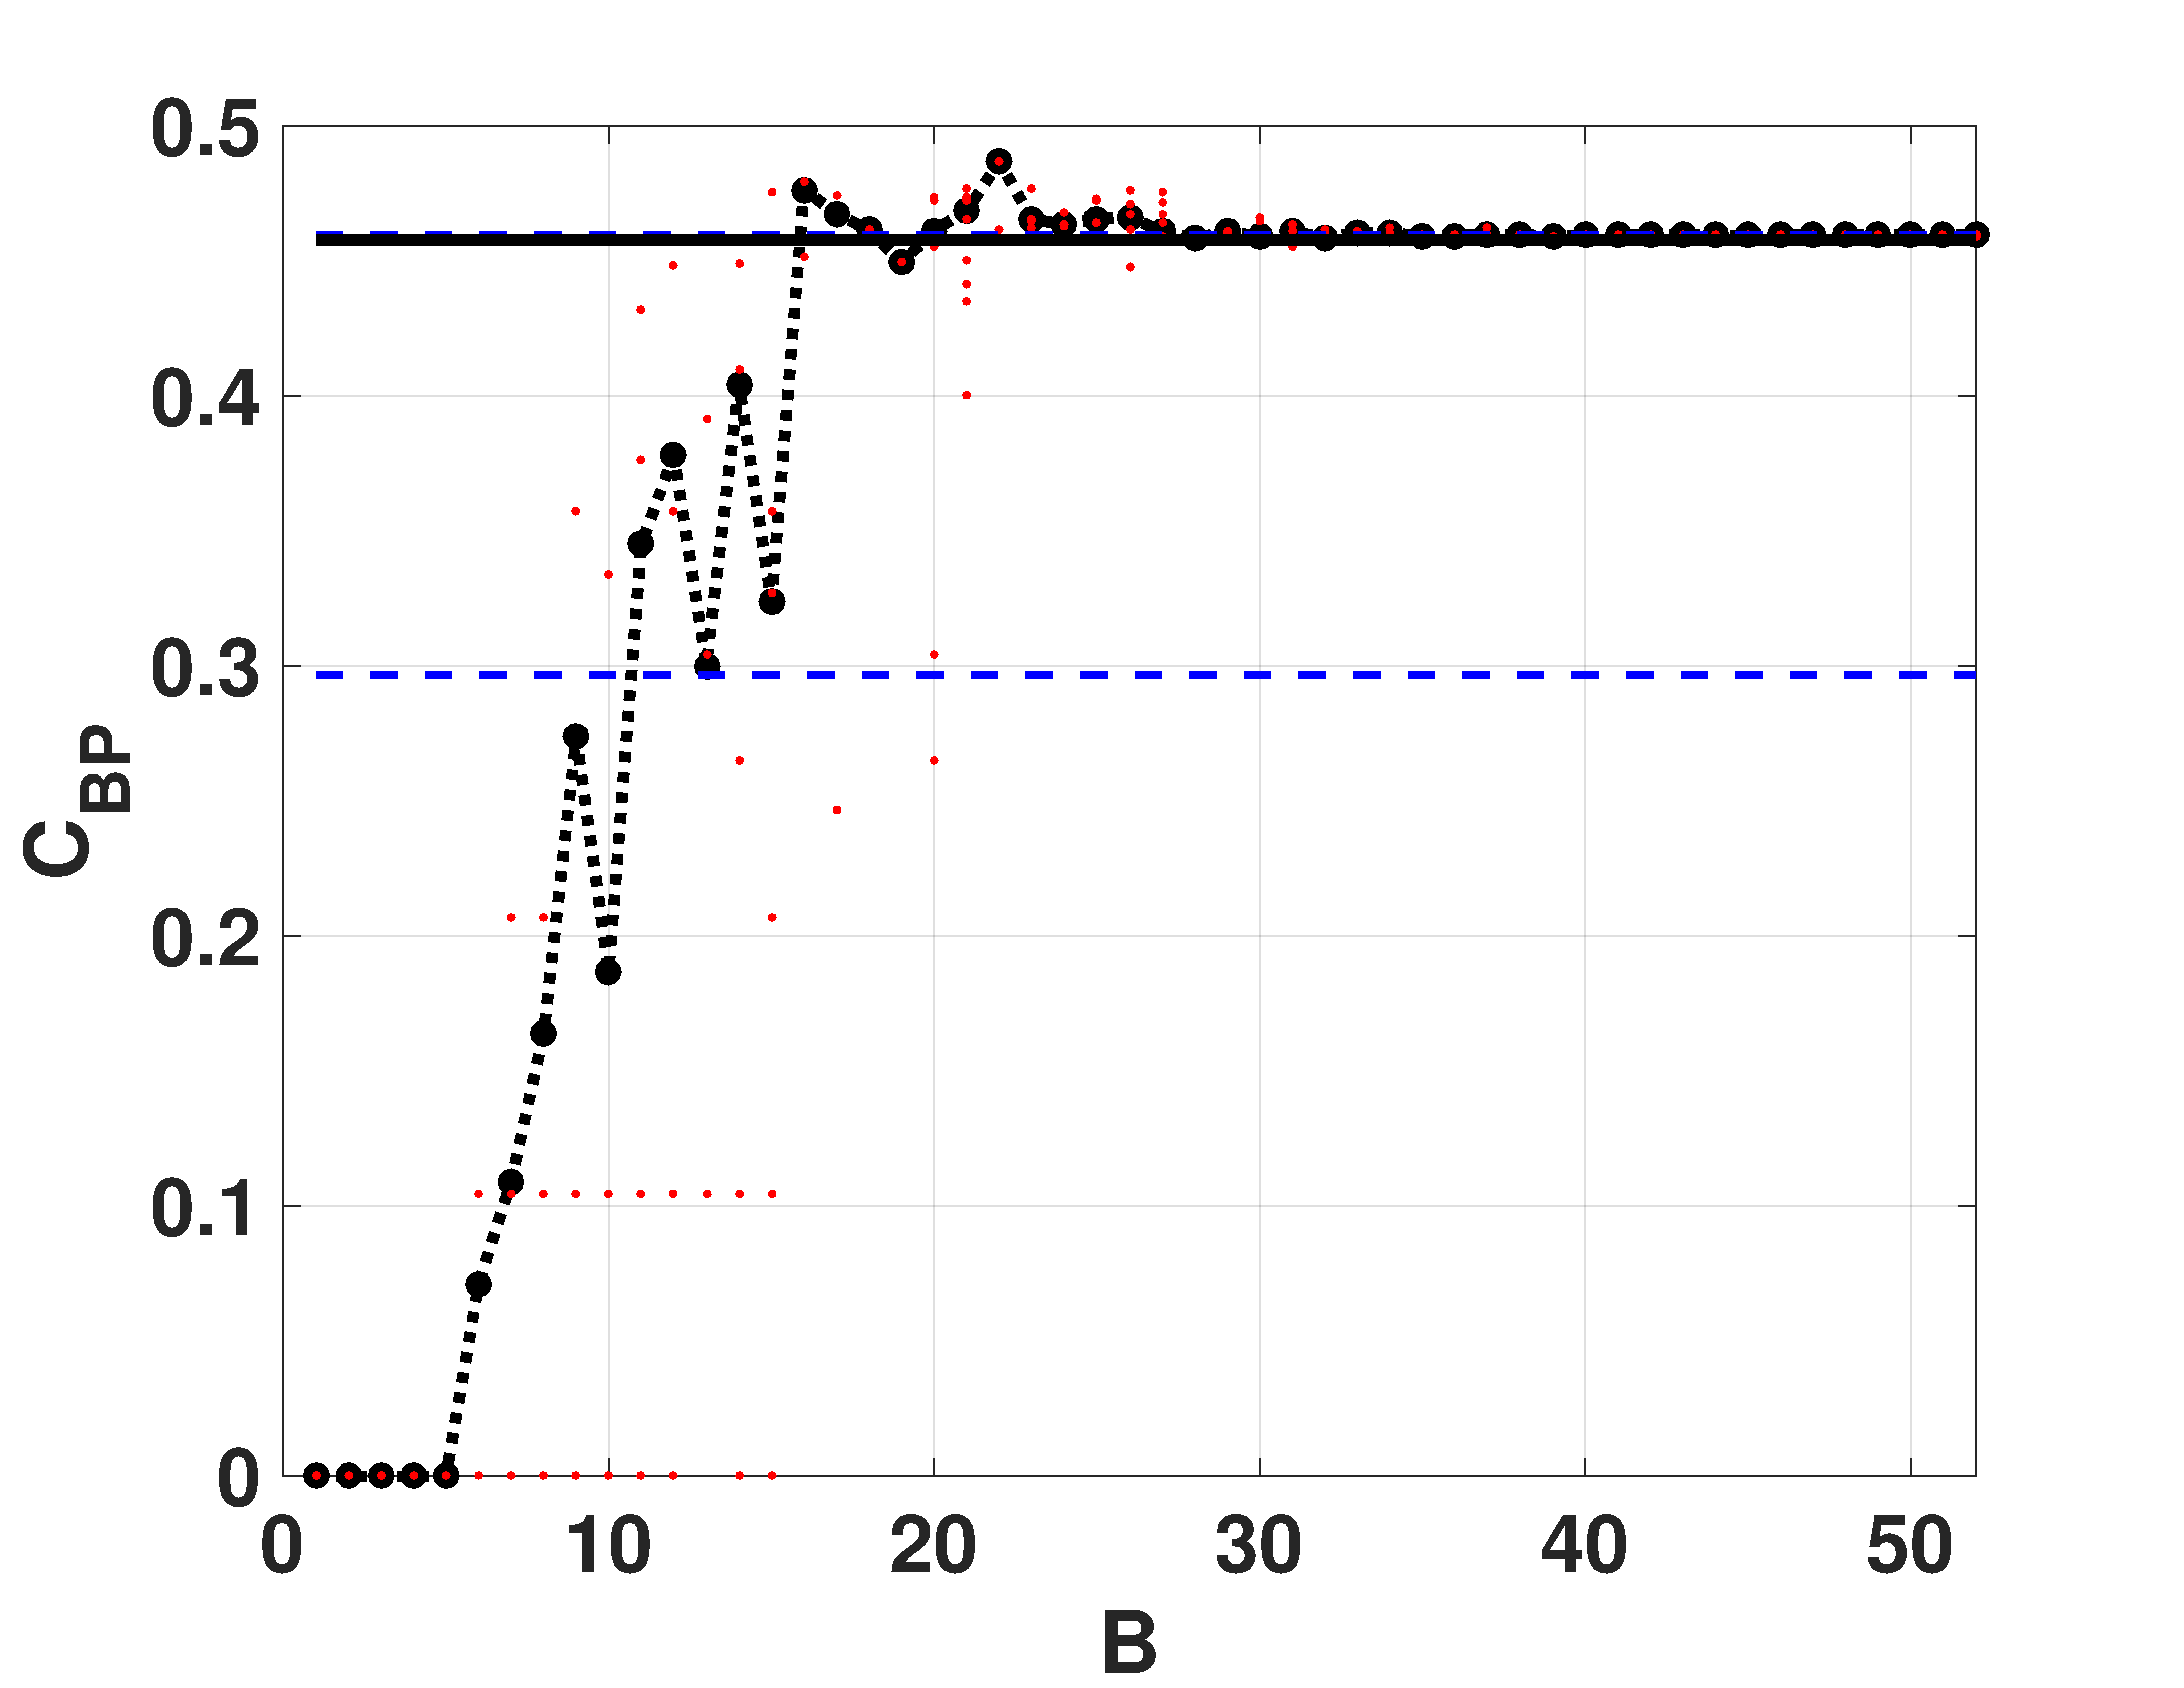
\includegraphics[width=\textwidth]{Cbp_Switch}
		\caption{$C_{BP}$ vs. $B$}
		\label{fig:Cbp_Switch}
	\end{subfigure}
	\begin{subfigure}[b]{0.49\textwidth}
		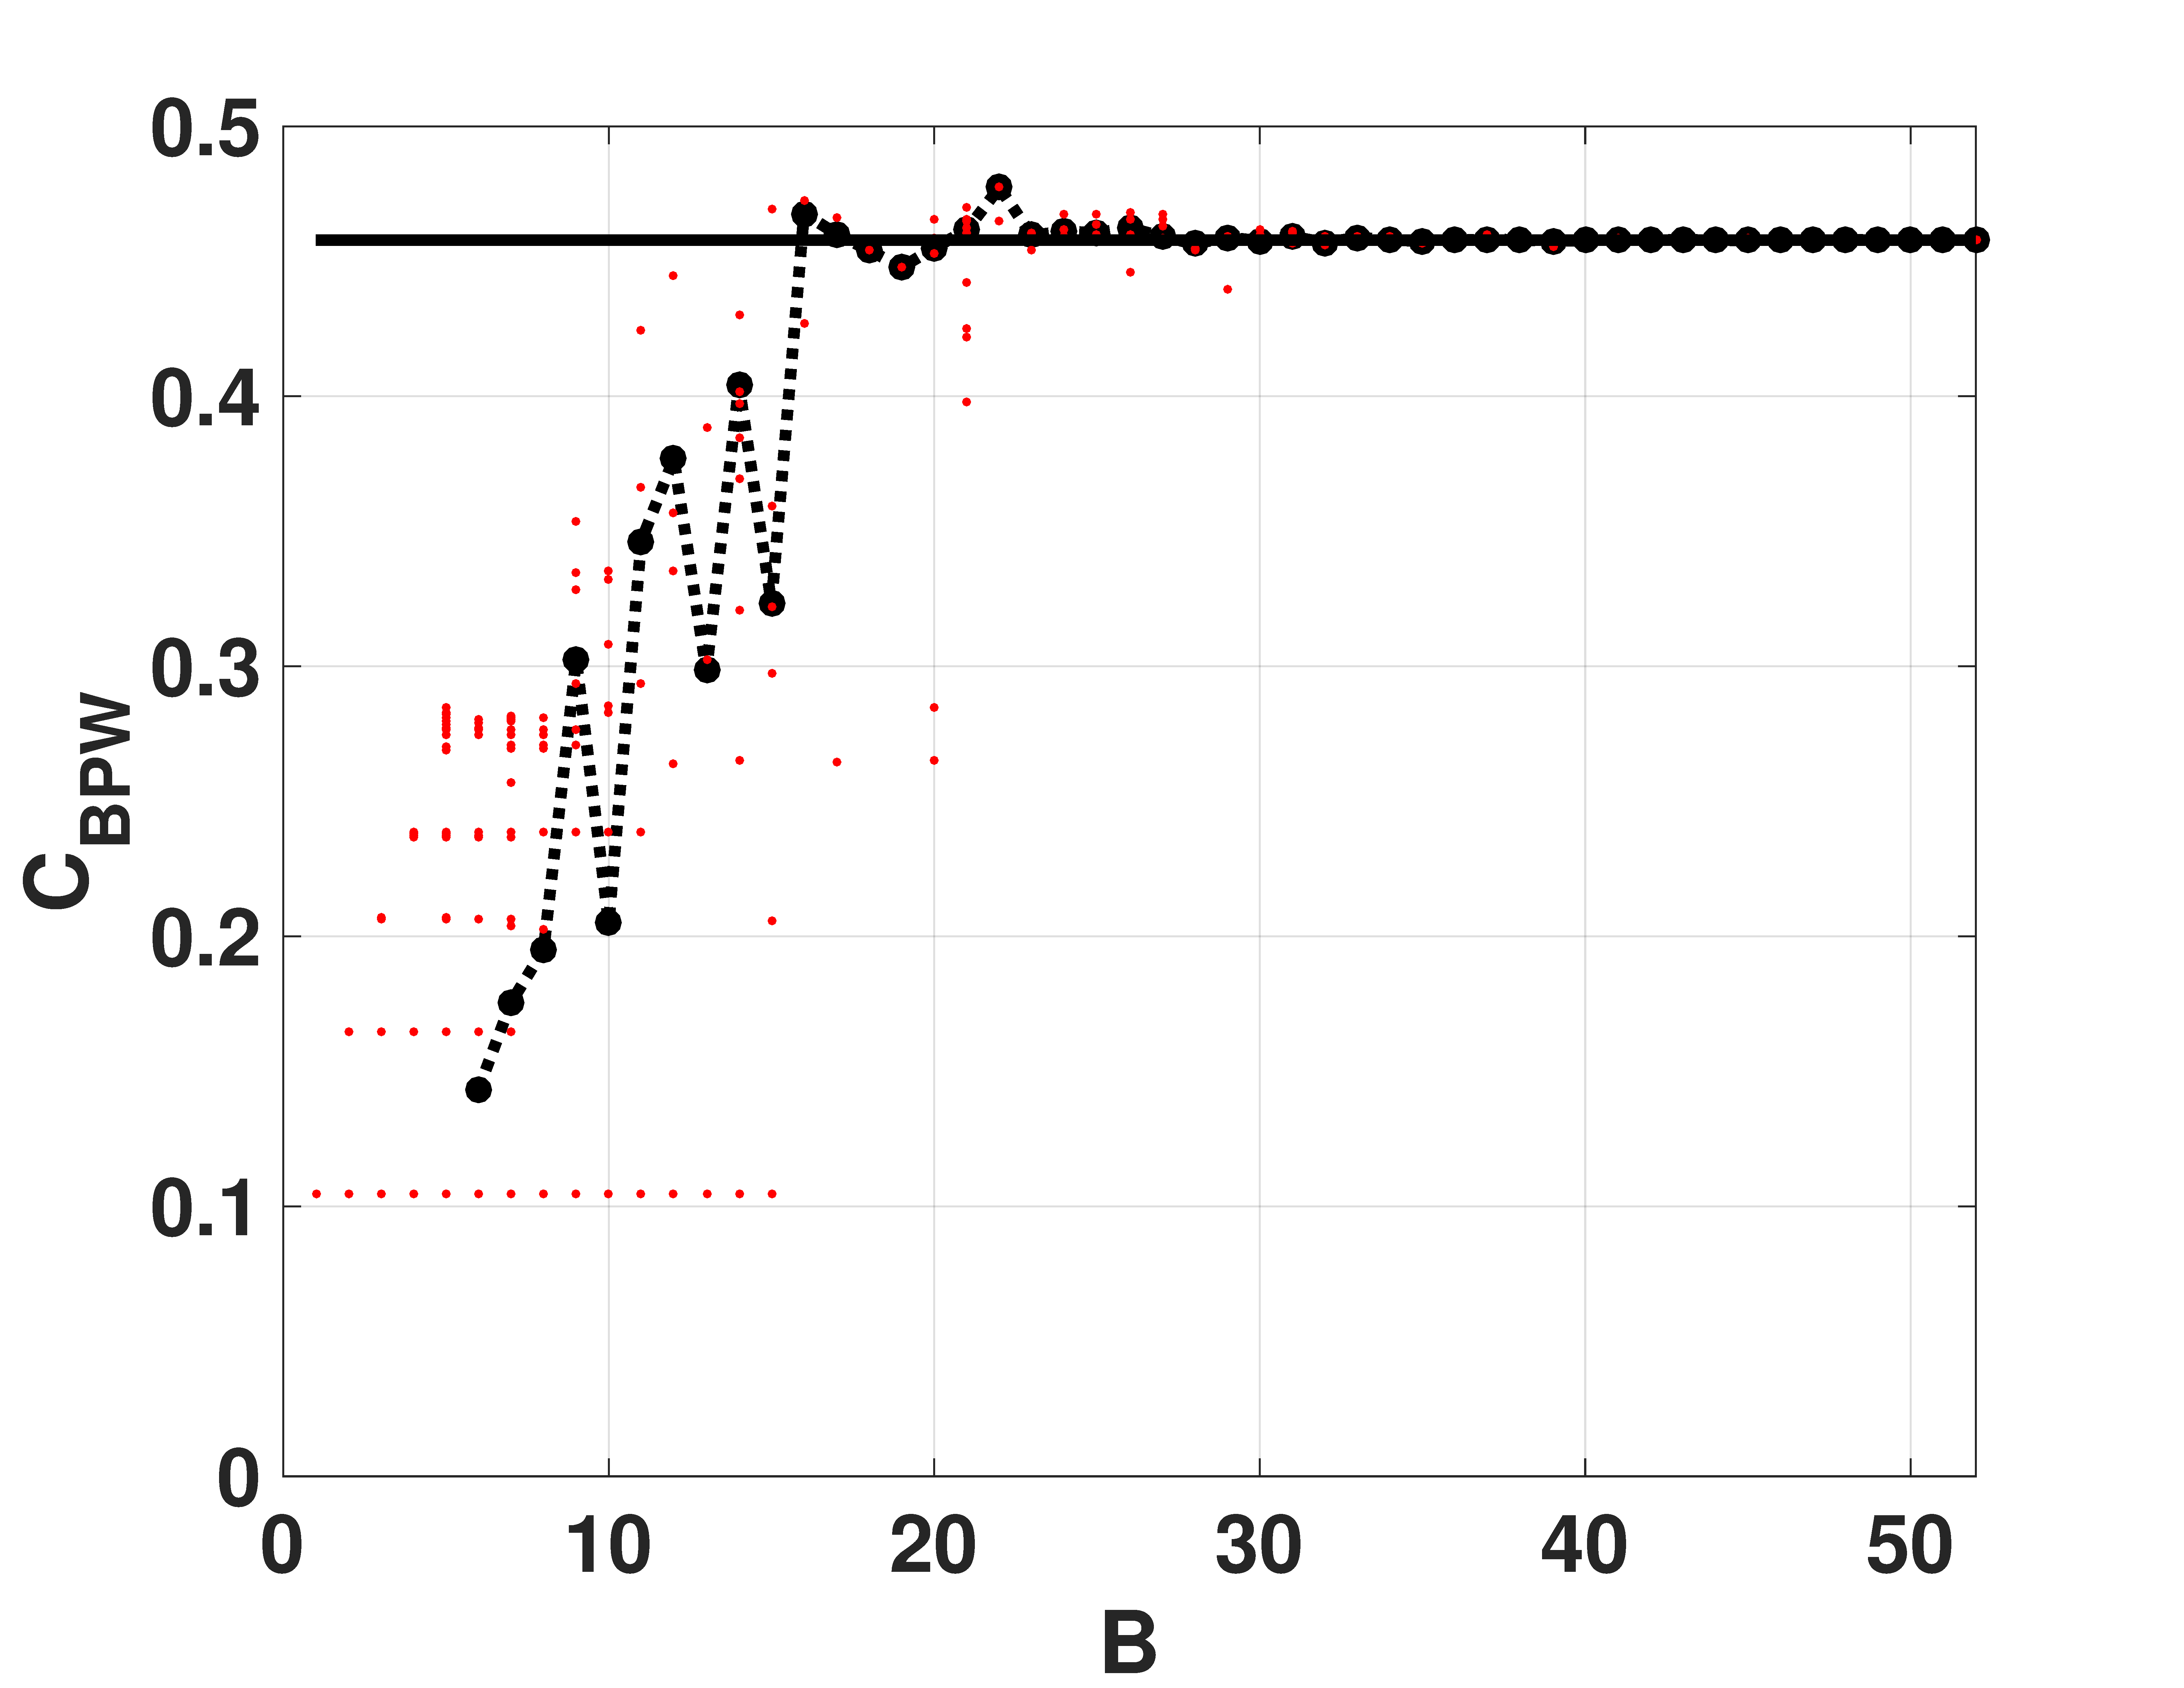
\includegraphics[width=\textwidth]{Cbpw_Switch}
		\caption{$C_{BPW}$ vs. $B$}
		\label{fig:Cbpw_Switch}
	\end{subfigure}
	\begin{subfigure}[b]{0.49\textwidth}
		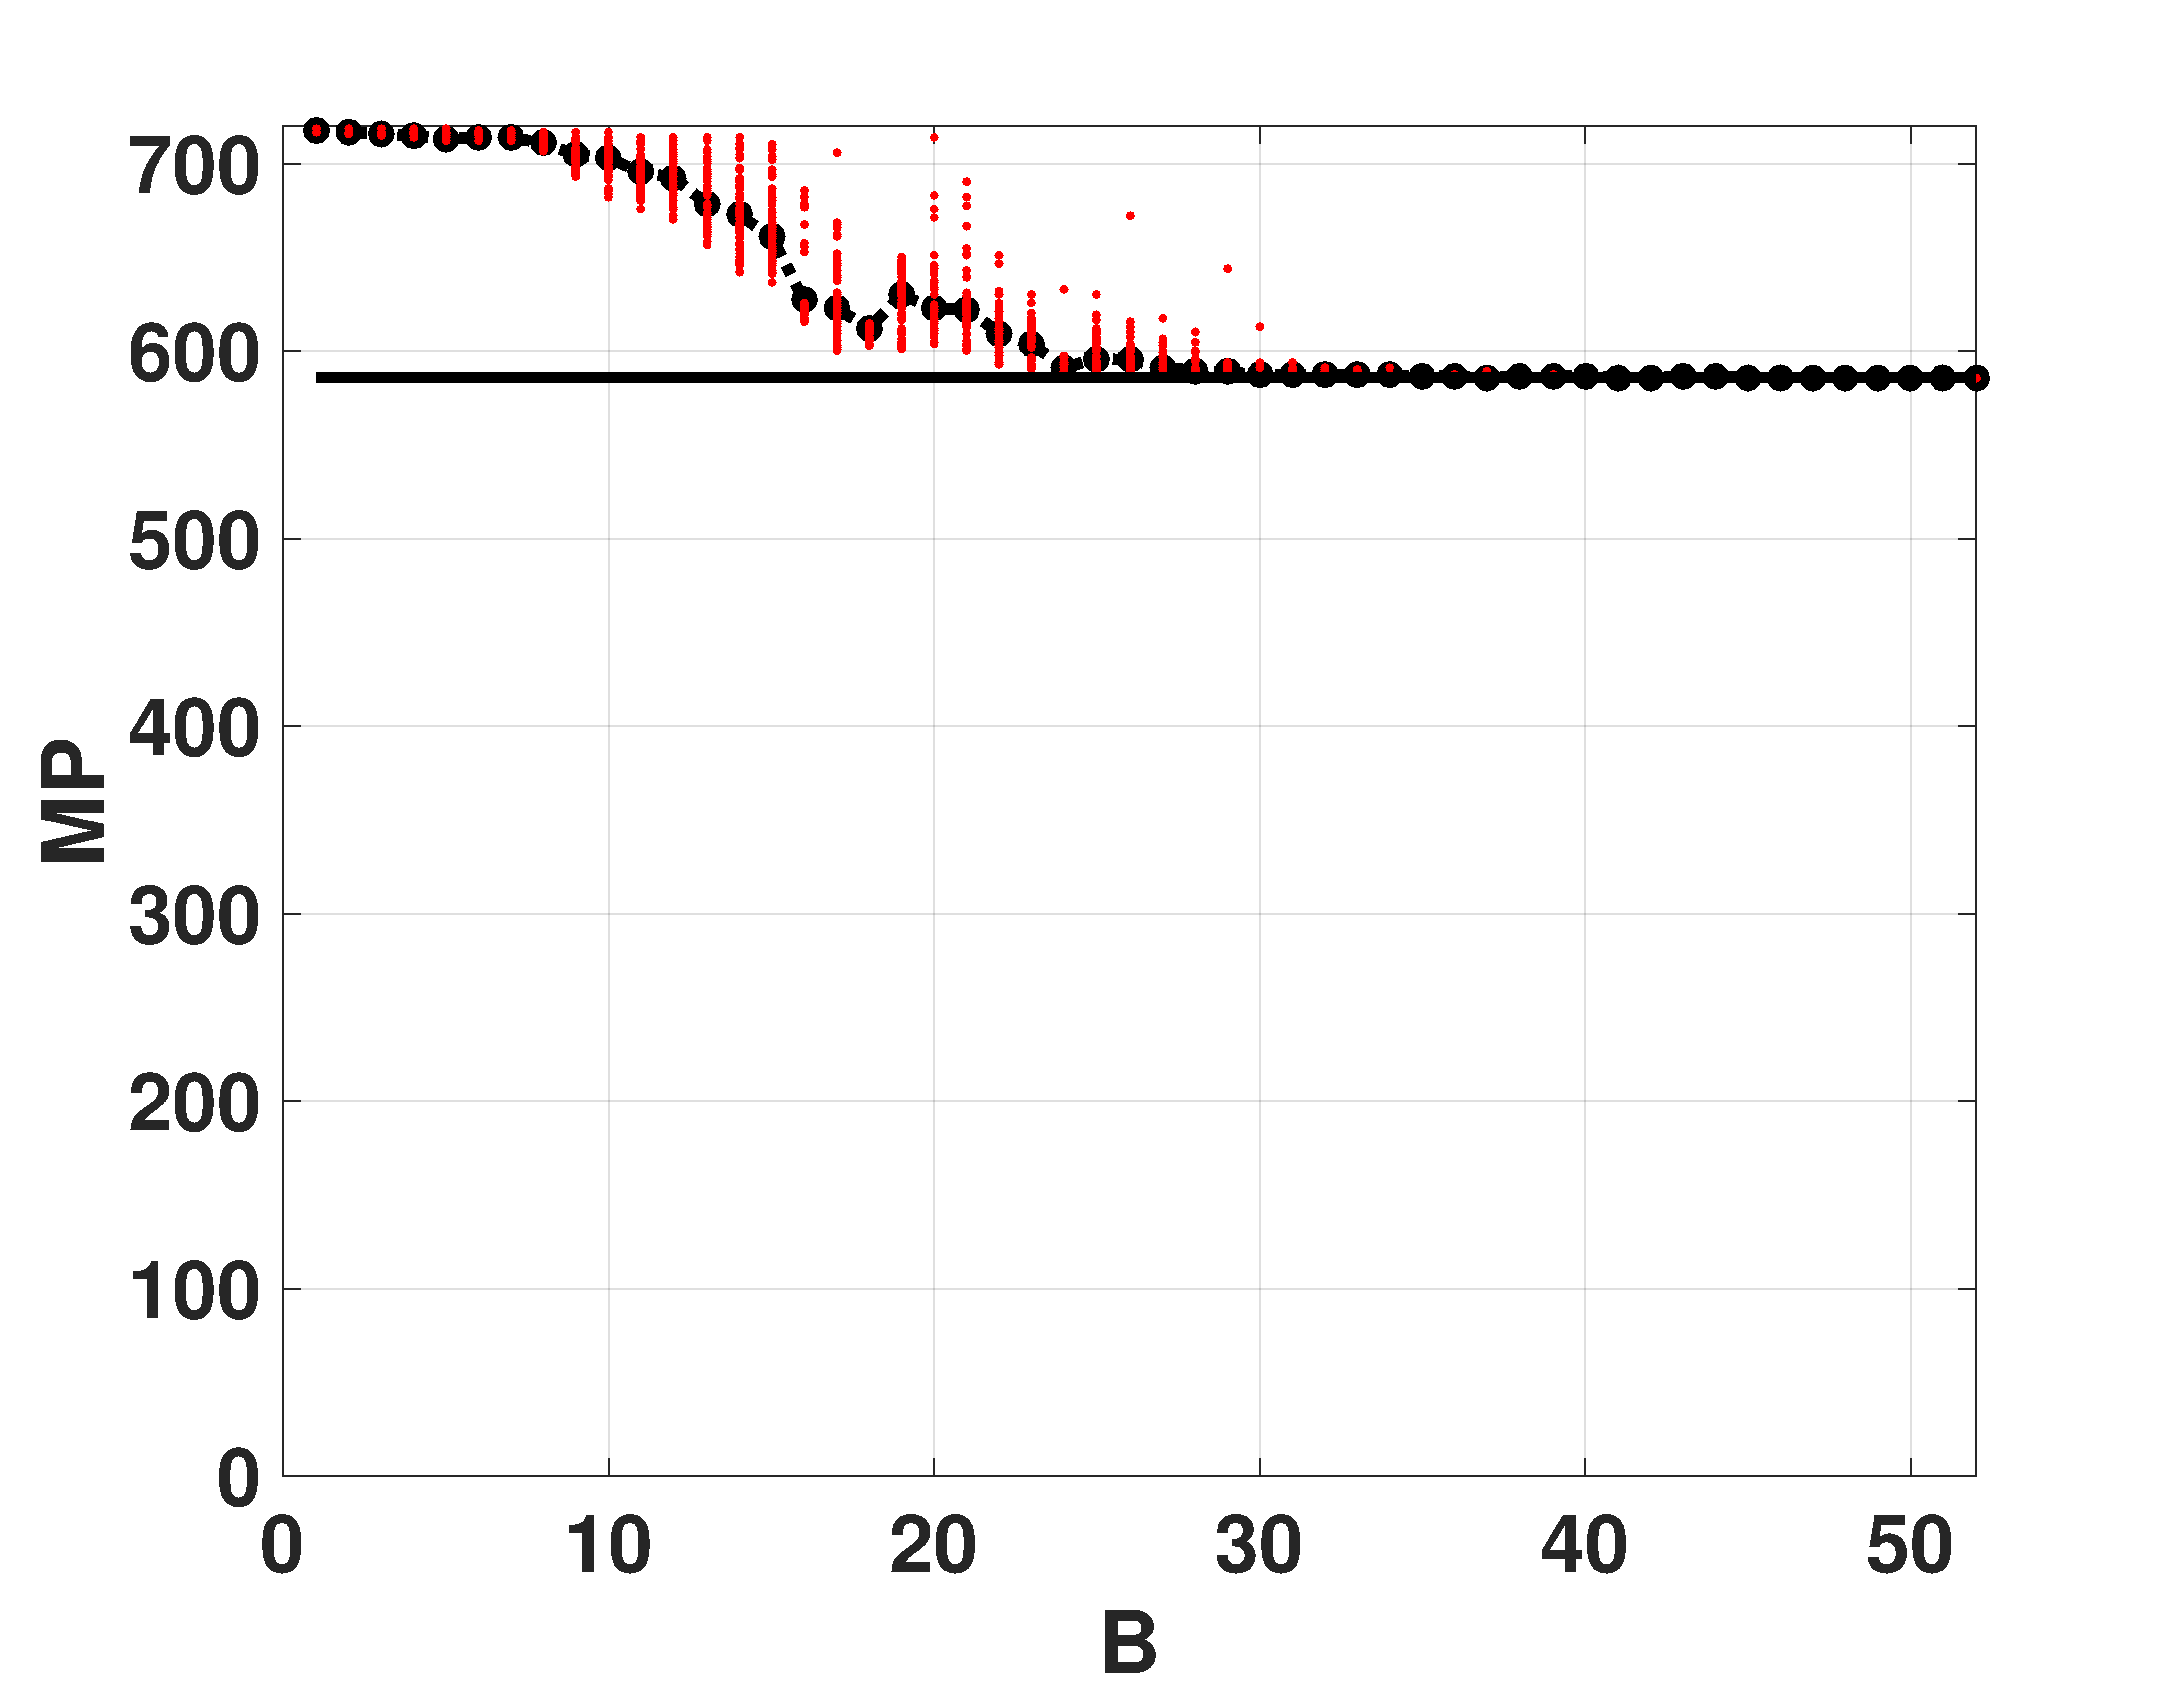
\includegraphics[width=\textwidth]{MP_Switch}
		\caption{MP vs. $B$}
		\label{fig:MP_Switch}
	\end{subfigure}
	\caption{Propiedades estadísticas del mapa SWITCH}
	\label{fig:SWITCH_QuantiB}
\end{figure}

El plano de doble entropía $H_{hist} \times H_{BP}$ se muestra en la Fig. \ref{fig:SWITCH_HH}.
El punto alcanzado en este plano para el mapa SWITCH es similar al alcanzado para el mapa LOG, y se indica con una estrella en la figura.
La mezcla es levemente mejor en este caso.
%
\begin{figure}[htpb]
	\centering
	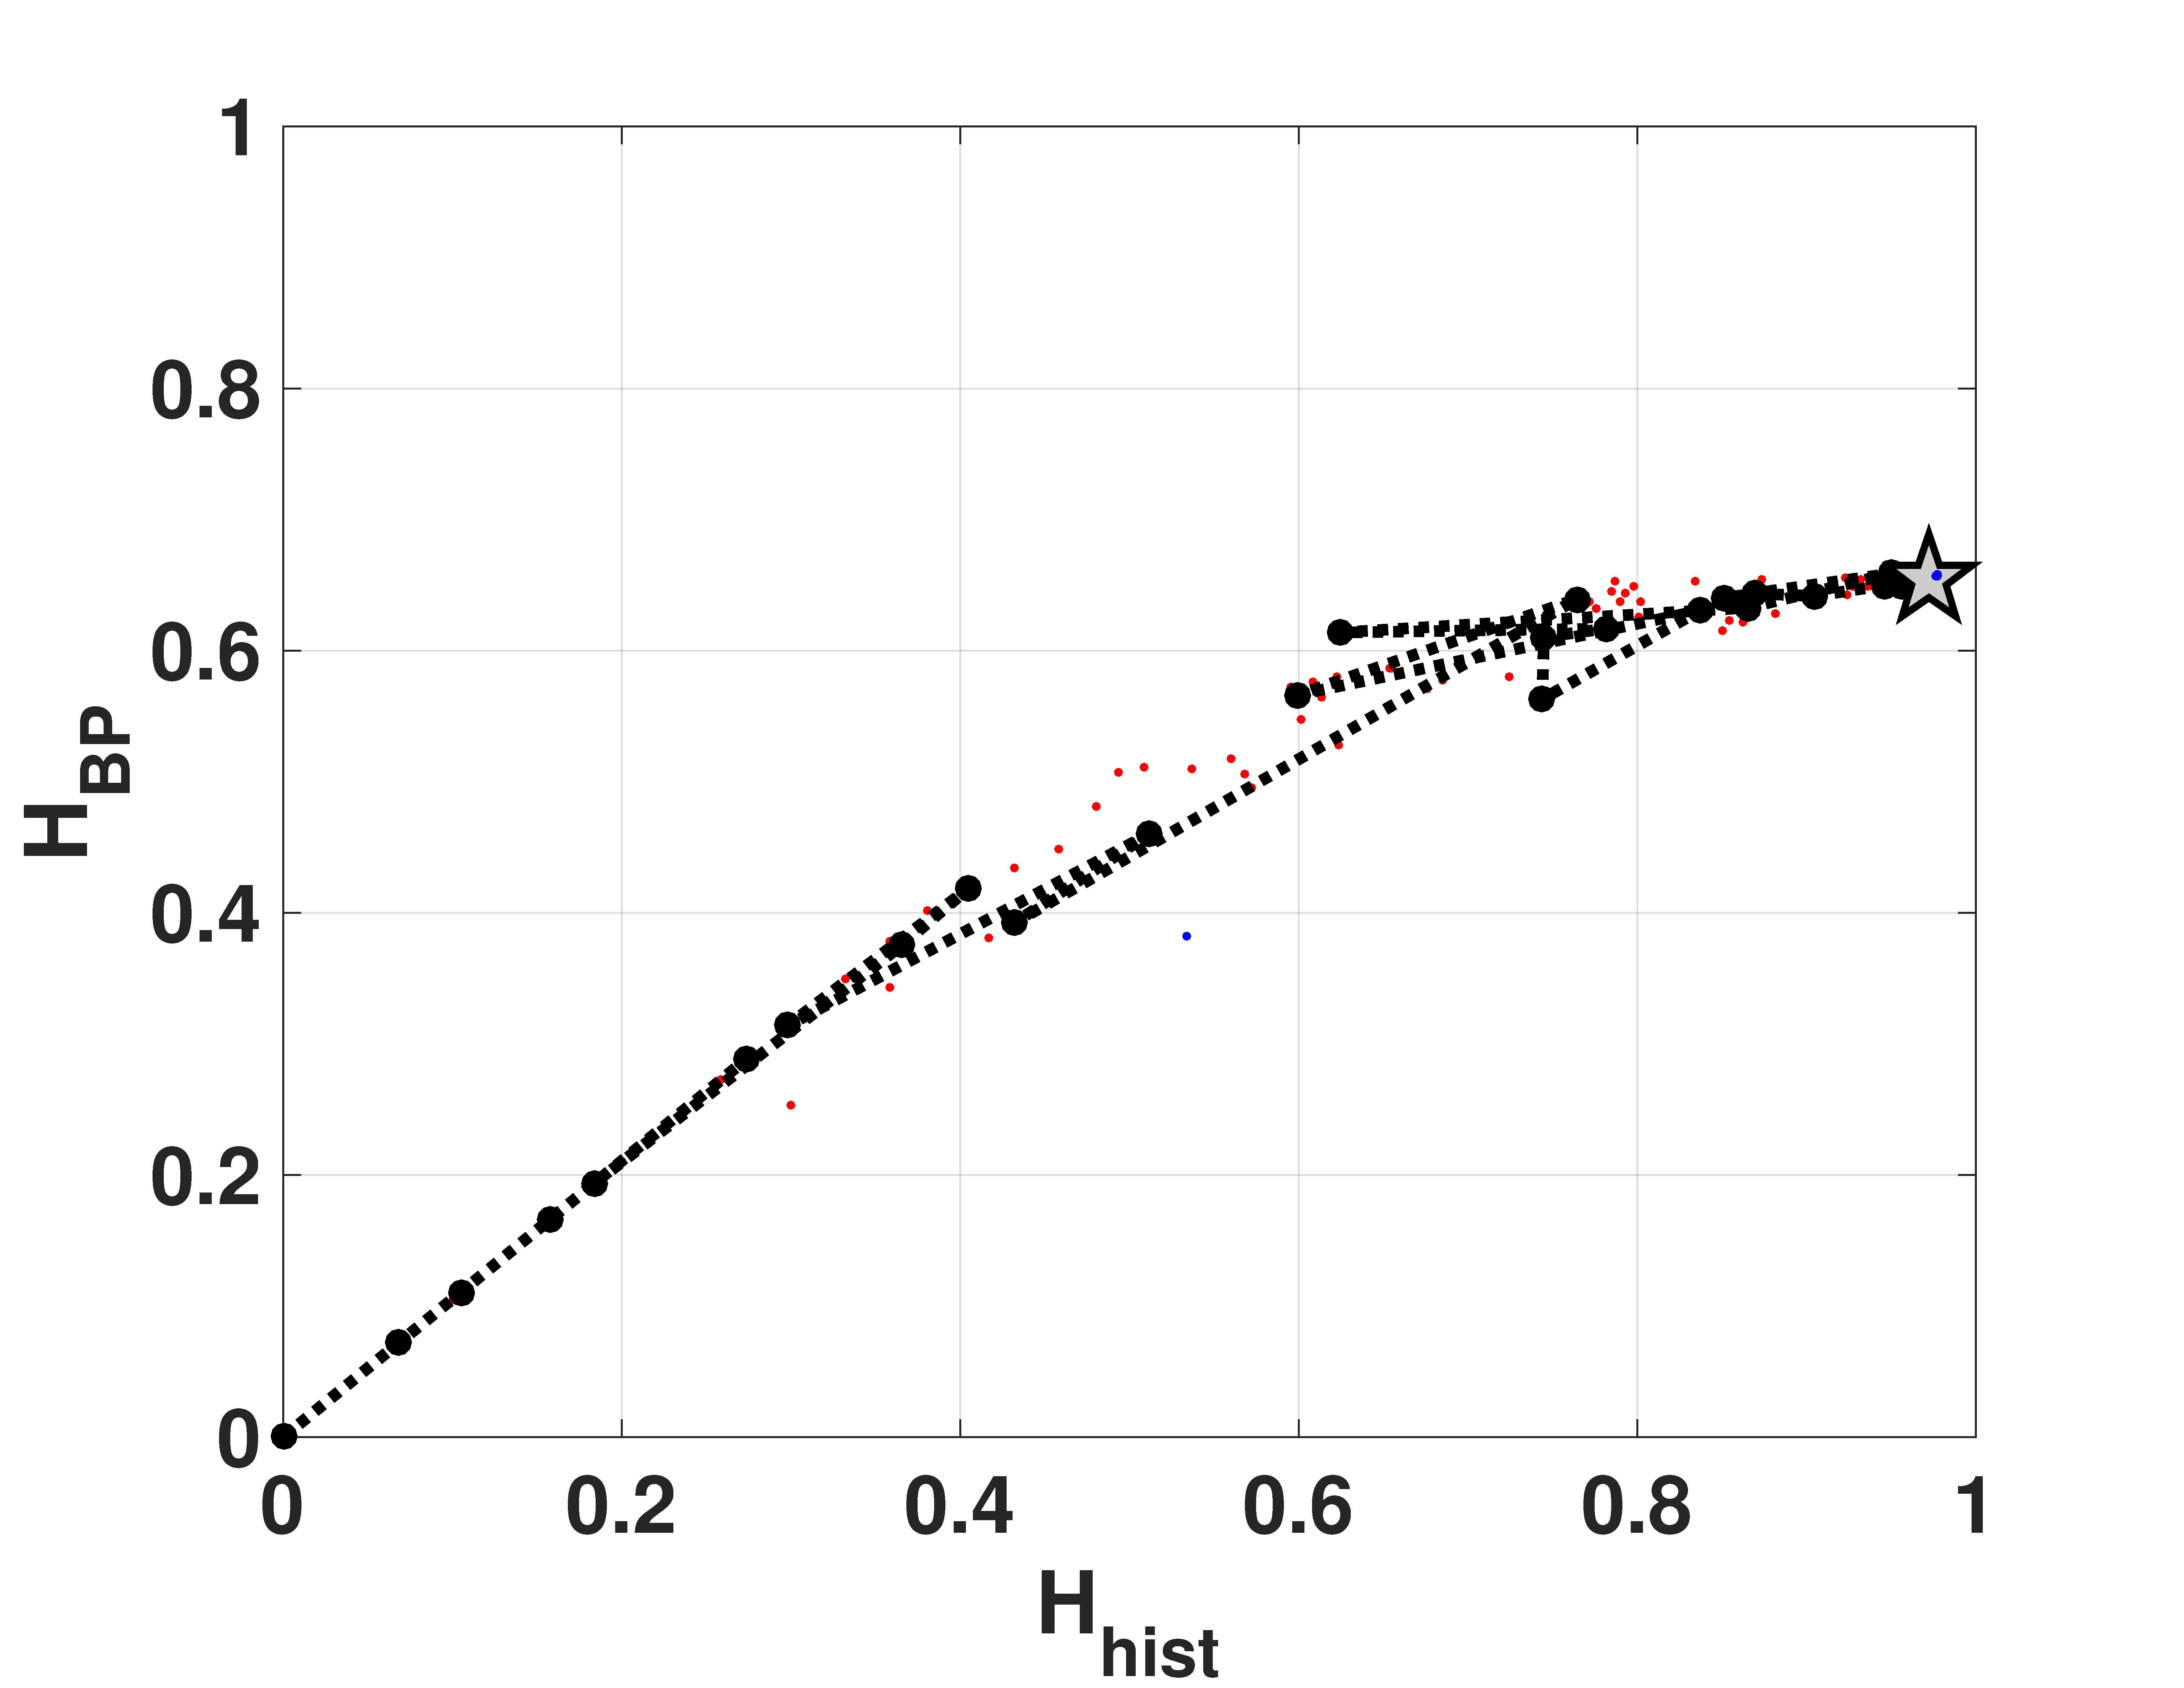
\includegraphics[width=.49\textwidth]{HbpHval_Switch}
	\caption{Evolución de las propiedades estadísticas en el plano doble entropía para el mapa SWITCH $H_{hist} \times H_{BP}$.}
	\label{fig:SWITCH_HH}
\end{figure}

El plano de entropía - complejidad $H_{BP} \times C_{BP}$ se muestra en la Fig. \ref{fig:SWITCH_HC}.
Si comparamos con el mismo plano en el caso de LOG (Fig. \ref{fig:CbpHbp_Log}), $C_{BP}$ es menor para SWITCH, este hecho muestra un comportamiento más aleatorio.
%
\begin{figure}[htpb]
	\centering
	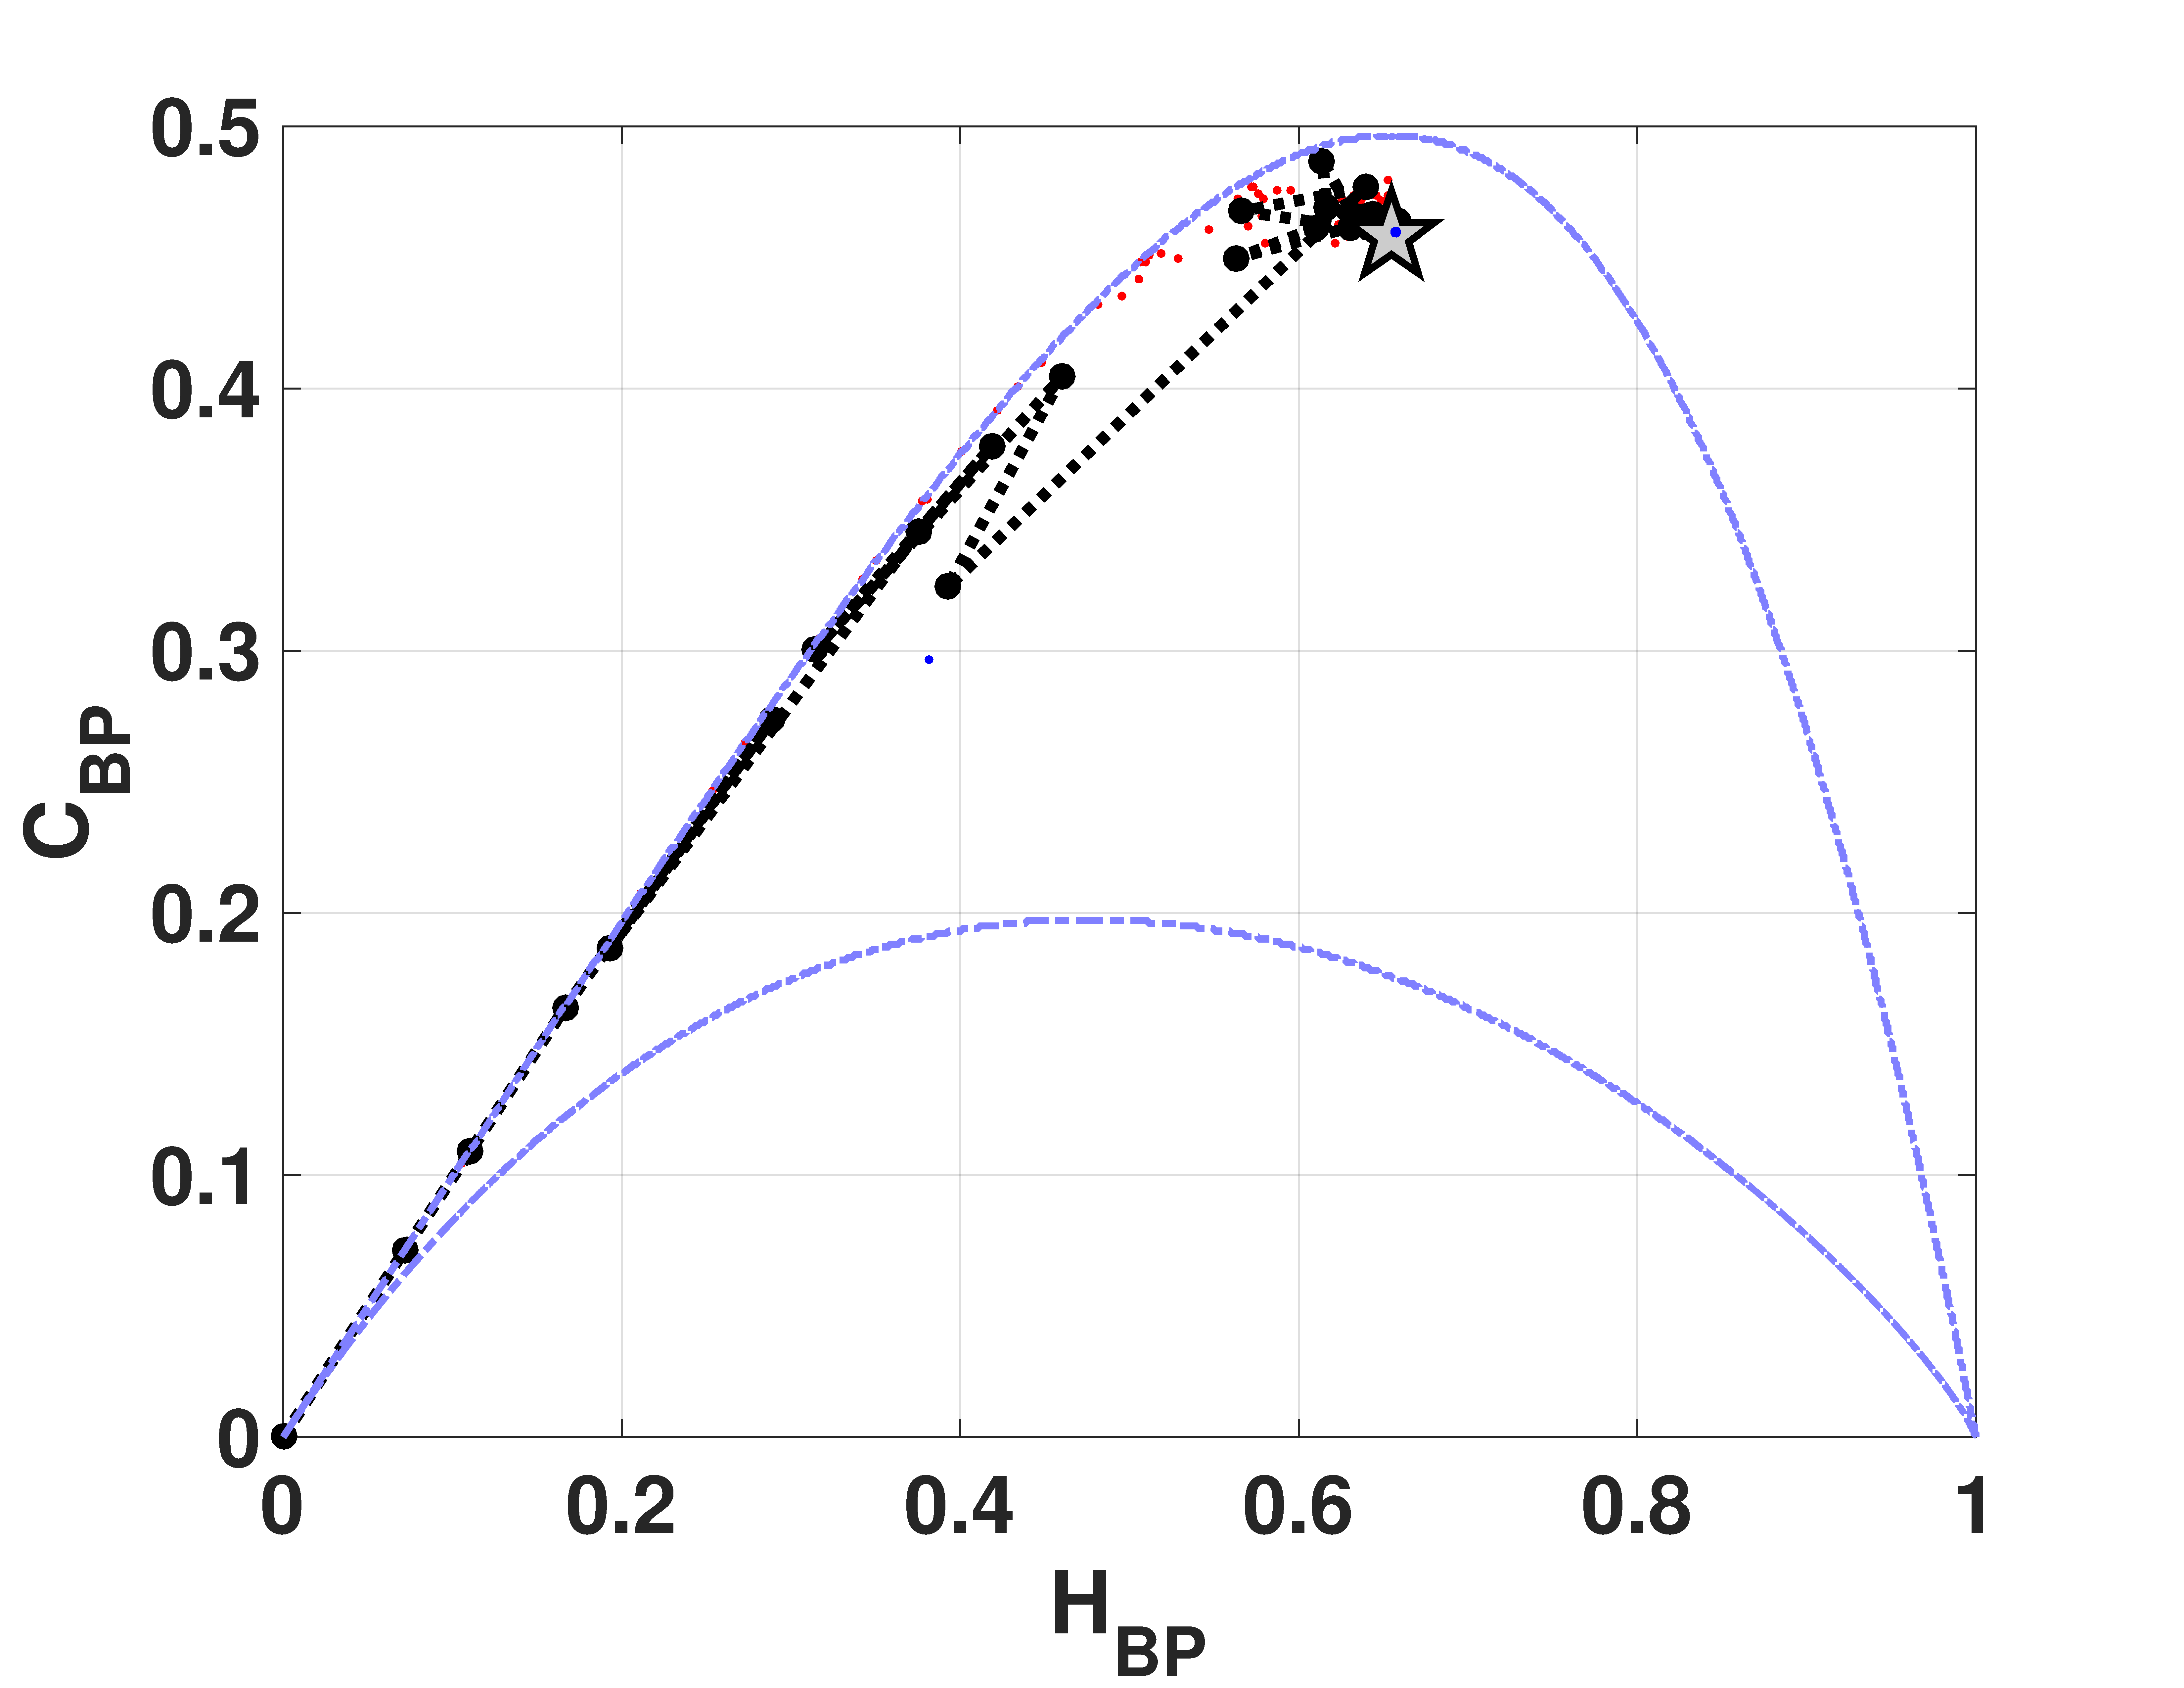
\includegraphics[width=.49\textwidth]{CbpHbp_Switch}
	\caption{Evolución de las propiedades estadísticas en el plano entropía - complejidad para el mapa SWITCH $H{BP} \times C_{BP}$.}
	\label{fig:SWITCH_HC}
\end{figure}